\documentclass{article}

\usepackage{arxiv}

\usepackage[utf8]{inputenc} % allow utf-8 input
\usepackage[T1]{fontenc}    % use 8-bit T1 fonts
\usepackage{hyperref}       % hyperlinks
\usepackage{url}            % simple URL typesetting
\usepackage{booktabs}       % professional-quality tables
\usepackage{amsfonts}       % blackboard math symbols
\usepackage{nicefrac}       % compact symbols for 1/2, etc.
\usepackage{microtype}      % microtypography
\usepackage{cleveref}       % smart cross-referencing
\usepackage{lipsum}         % Can be removed after putting your text content
\usepackage{graphicx}
\usepackage[english]{babel}
\usepackage[
backend=biber,
style=alphabetic,
sorting=ynt
]{biblatex}
\usepackage{doi}
\usepackage{placeins}
\addbibresource{references.bib}
\title{GPU Memory Harvesting for Global Memory Cache in Deep Learning Clusters}

% Here you can change the date presented in the paper title
%\date{September 9, 1985}
% Or remove it
%\date{}

\newif\ifuniqueAffiliation
% Uncomment to use multiple affiliations variant of author block 
\uniqueAffiliationtrue

\ifuniqueAffiliation % Standard variant of author block
\author{Anmol Agarwal \\
	Masters in Computer Science\\
	Georgia Institute of Technology\\
	\texttt{aagarwal622@gatech.edu} \\
	%% examples of more authors
	\And
	Hersh Dhillon \\
	Masters in Computer Science\\
	Georgia Institute of Technology\\
	\texttt{hdhillon30@gatech.edu} \\
	\And
	Prakhar Jagwani \\
	Masters in Computer Science\\
	Georgia Institute of Technology\\
	\texttt{pjagwani3@gatech.edu} \\
	%% \And
	%% Coauthor \\
	%% Affiliation \\
	%% Address \\
	%% \texttt{email} \\
	%% \And
	%% Coauthor \\
	%% Affiliation \\
	%% Address \\
	%% \texttt{email} \\
}
\else
% Multiple affiliations variant of author block
\fi

% Uncomment to override  the `A preprint' in the header
\renewcommand{\headeright}{Technical Report - CS 8803-SMR}
\renewcommand{\undertitle}{Technical Report - CS 8803-SMR}
\renewcommand{\shorttitle}{\textit{arXiv} Template}

%%% Add PDF metadata to help others organize their library
%%% Once the PDF is generated, you can check the metadata with
%%% $ pdfinfo template.pdf
\hypersetup{
pdftitle={A template for the arxiv style},
pdfsubject={q-bio.NC, q-bio.QM},
pdfauthor={David S.~Hippocampus, Elias D.~Striatum},
pdfkeywords={First keyword, Second keyword, More},
}

\begin{document}
\maketitle

\begin{abstract}
The computational capacity of GPUs has been increasing over the past recent years, however, the memory capacity
has remained almost the same. On the other hand, both the compute and memory requirements of
models has been increasing steadily over over the years. This makes the GPU memory a 
precious resource while training deep learning models. Hence there is need for 
Memory Harvesting of GPUs to allow training large models despite memory contraints. We
currenlty focus on harvesting memory on a single GPU and then can extend to multi-GPU scenario.
We also demonstrate how we perform eviction, prefetching of tensors and measure the overhead
of Ravenstore when training models.
\end{abstract}


% keywords can be removed
\keywords{Memory Harvesting \and Caching \and Prefetching \and Offloading}


\section{Introduction}
\subsection{Motivation}
Our Memory Harvesting technique is meant to help large models train on GPUs with limited capacity.
We leverage the following key insights in order to help define our design goals:
	\subsubsection{Limited Memory Growth}As shown in figure <REF>, for state of 
	art GPUs, there is drastic increase in TeraFLOPS across different GPUs, but memory increase is negligible.
	This implies that we might be able to meet compute requirements of the models better than their memory requirements.
	Hence, there is a need for a way to address the issue of limited memory without hampering model's training and performance.
	\begin{figure}[!htbp]
		\centering
		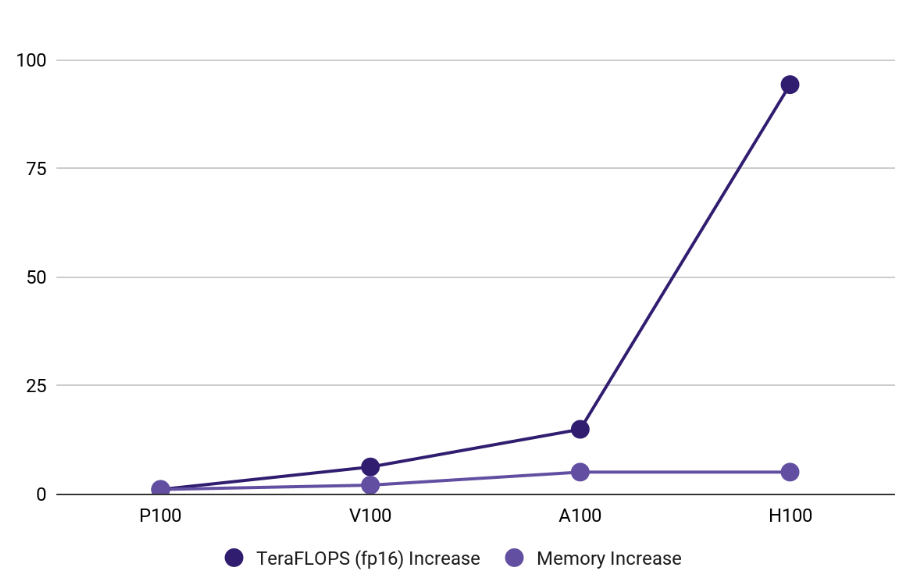
\includegraphics[height=4cm, width=6cm]{figures/teraflops.png}
		\caption{GPU FLOPS vs Memory Growth}
	\end{figure}

	\subsubsection{Highly Skewed Memory Utilization}
	Even though workloads suffer from memory bottlenecks, several studies have shown that, in production clusters, memory utilization
	is suboptimal. For example, as shown in figure <REF>, in Alibaba's production cluster, only 20\% of GPUs have applications
	utilizing over 80\% of their memory. There is need to harvest underutilized GPUs to support applications requiring 
	higher amount of GPU memory than is available.
	\begin{figure}[!htbp]
		\centering
		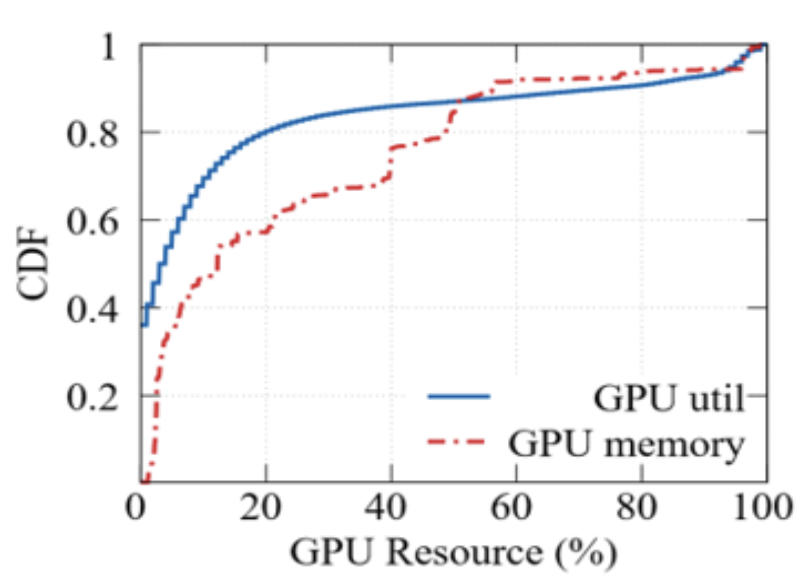
\includegraphics[height=5cm, width=6cm]{figures/AlibabaUtil.png}
		\caption{GPU Memory Utilization in Alibaba's Production Cluster}
	\end{figure}
	\FloatBarrier

	\subsubsection{Naive Eviction/Prefetching Policies} In other to swap tensors out to GPU memory to give space for other tensors needed by application,
	policies like LRU can be used to decide what tensors to evict. However, these policies are naive because they don't take into account the following two factors:
	\begin{itemize}
		\item \textbf{Heterogeneous Size of Tensors}: LRU policy might only evict tensor which was least recently used. However, 
		if the size of this tensor was in KBs, it could have done better by evicting a larger tensor (whose size is in MBs/GBs) instead. Similarly,
		LRU might swap out a very large tensor (running into GBs) to make space a small tensor whose size maybe in bytes.
		\item \textbf{Latency Awareness}: The pattern of usage of tensors is quite predictive when training models [Potential Citation], and the pattern is repetitive. For example,
		when training a deep neural network, we can offload activations generated at each layer to CPU because they are not going to be required before backward propagation phase.
		Now, since we know that activations which were generated most recently (i.e. from last layer), would be needed first.
		A smart prefetching policy will know this pattern, and decide to prefetch activations starting from the last layer.
	\end{itemize}

\subsection{Design Decisions}
With above issues in mind, we propose the following design decisions to mitigate these issues and maximize
the utility of the system. For the sake of interpretability, we will refer to tensors not managed by Ravenstore as those lying in
Userspace and those managed by Ravenstore as those lying in Ravenspace. Applications can only use tensors present in user space.
	\subsubsection{APIs}Clients/Applications are provided with the following four APIs to help manage tensors for memory harvesting purposes:
	\begin{itemize}
		\item \textbf{Create}: Whenever clients want new tensors, they can call create with specified size and Ravenstore will
		create space for those tensors.
		\item \textbf{Get}: Whenever clients need to use tensors, they can call get API specified with tensor id, so that those tensors
		move to Userspace (if they were present in Ravenspace) and clients can use them.
		\item \textbf{Put}: When clients don't need tensors, but might need them later (for example, activation tensors might be needed later during backward propagation phase),
		they can call put API to allow moving tensors back to Ravenspace and Ravenstore can do whatever it wants to ensure maximum GPU utilization and low latency.
		\item \textbf{Free}: When clients don't need tensors at all, they can call free API to delete the tensor.
	\end{itemize}
	\subsubsection{Abstraction}Whatever Ravenstore with Memory Harvesting does underneath with the tensors created by applications is completely
	unknown to them. Neither the applications should care about that. All they need is the following:
	\begin{itemize}
		\item Tensors must be available to them when they call get() API.
		\item All other APIs must work as expected without interfering with clients' program as well as the programs not managed by Ravenstore.
	\end{itemize}
	\subsubsection{Low Latency in Get API} When clients call get() when they need tensors for further computations on their GPU, Memory Harvesting implementation does the following:
	\begin{itemize}
		\item Check if tensor is already present on GPU device where the client is running.
		\item If tensor is not already present, then Ravenstore will fetch the tensor from CPU memory to GPU device.
		\item And the tensor would be moved to Userspace and handed over to the user.
	\end{itemize}
	The second step, i.e., when tensor is not already present on GPU, incurs high latency when moving the tensor to GPU.
	This will hugely increase training/inference time of models on the clients. In other to avoid that, we have prefetching mechanisms.
	Clients will need to specify the time they will need the tensors (through Put API) again in future, and Memory Harvesting framework will
	fetch those tensors beforehand if possible to avoid delays in Get() API call.

\section{Related Work}
\cite{shuklasingularity}

Recent deep learning training systems built for training large language models like ZeRO [1, 2] and FSDP [3, 4] use sharding and offloading of 
GPU memory to CPU memory or NVMe drives to reduce the active memory pressure in DL workloads. However, these solutions are highly customized 
for specific workloads and require non-trivial engineering efforts to support new applications. Systems like GPUSwap [12]  and CUDA unified 
memory [8]  can be utilized to build a general-purpose offloading system, however, these systems utilize simple cache eviction strategies 
like random or LRU and not take advantage of the predictable access patterns of DL workloads.

There are other works that implementation offloading. Accelerate is a library available on huggingface that does layer by layer offloading 
which helps in training large models where atleast one layers fits in the GPU memory at a time. ZeRO-Infinity introduces a novel GPU memory 
optimization technique called memory-centric tiling to support extremely large individual layers that would otherwise not fit in GPU memory 
even one layer at a time.

While they are all great works, they are all limited to one DL process at a time, not the entire GPU. These can lead to starvation of other
GPU processes since they take as much GPU as possible before. We show that our solution handles this on the GPU level and provides a
way to handle multiple processes without starvation.


\section{High Level Design}
\begin{figure}[!htbp]
	\centering
	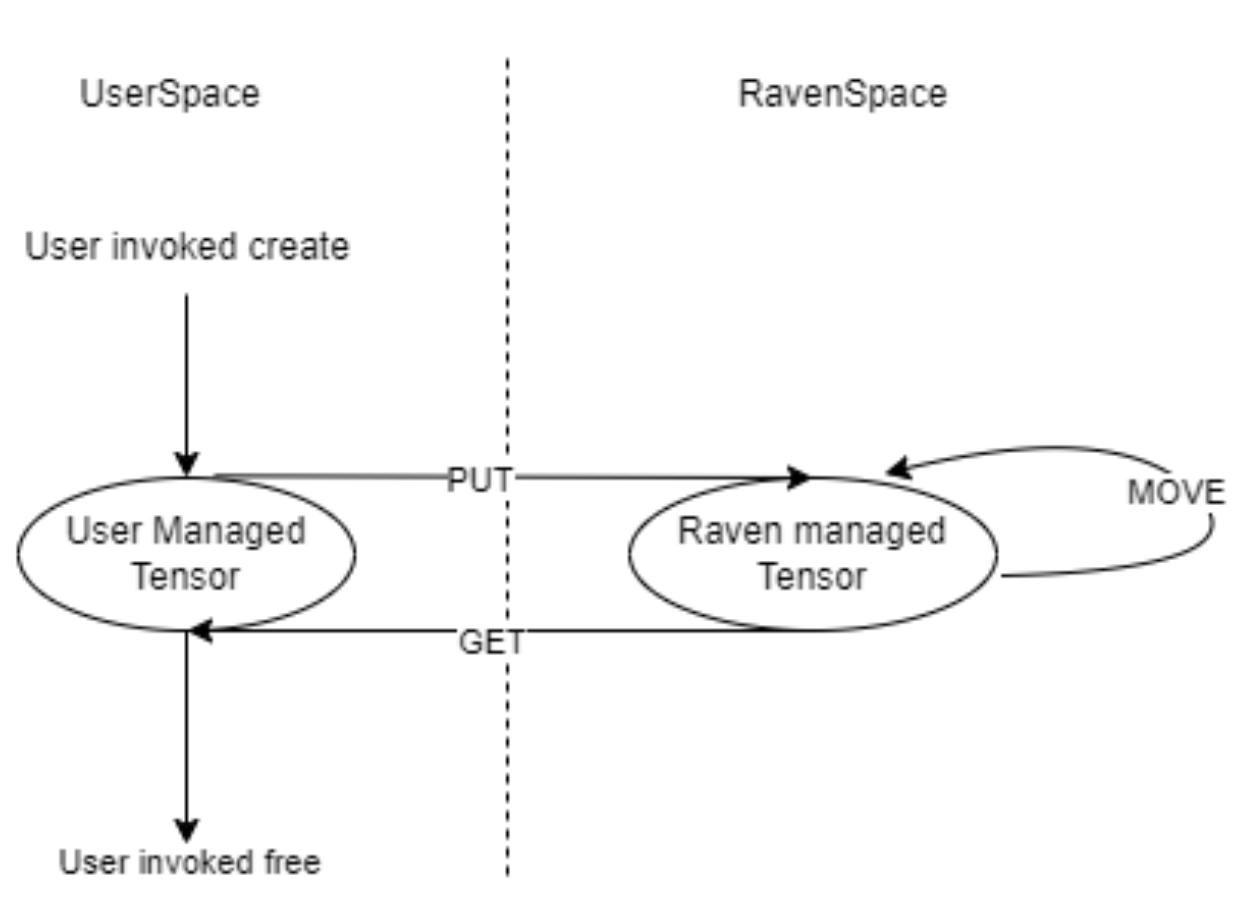
\includegraphics[height=6cm, width=8cm]{figures/ravenspace.png}
	\caption{A visual description of Userspace and Ravenspace}
\end{figure}
We divide the space in which our tensors exist into two partitions, Userspace and Ravenspace.
Whenever a tensor is created, it is created in the Userspace. By default all intercepted mallocs 
are allocated in the Userspace. The tensors in the Userspace are not managed by Ravenstore. 
The tensors allocated in the Userspace will continue to be in the GPU and accessible the handle to 
the tensor until it is explicitly freed by the User.

Ravenspace on the other hand is managed by Ravenstore. Once a tensor is put into Ravenspace the user
can only access it again once they call the get API. The get API will bring the tensor back to the GPU if it was evicted
and then back in the Userspace where the user can use the handle to access the tensor. Hence, tensors in 
Ravenspace are immutable.

Tensor in the Userspace are first class citizens of the system i.e. if we find that the GPU memory is full,
we will offload the tensors from the Ravenspace to make room for them. If we still cannot allocate a tensor in Userspace,
means that we are out of GPU memory and user has to free some of their tensors to make room.

\begin{figure}[!htbp]
	\centering
	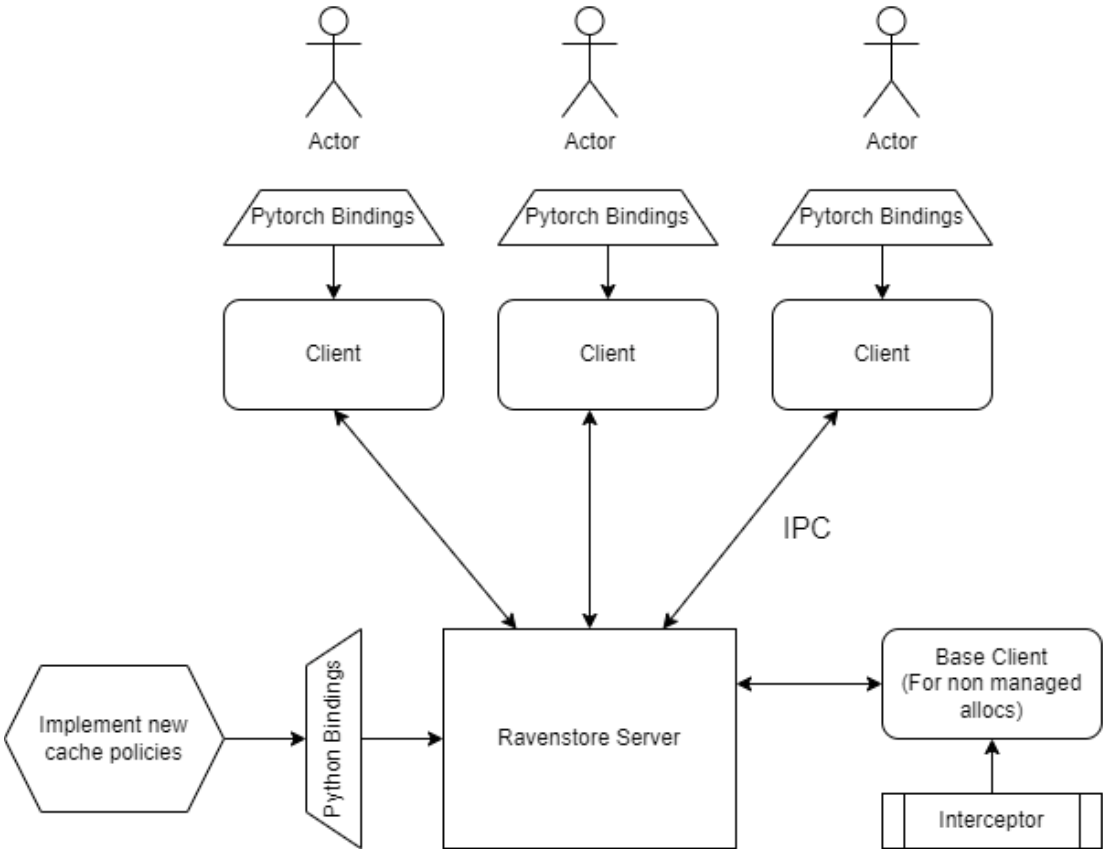
\includegraphics[height=6cm, width=7cm]{figures/hld.png}
	\caption{High Level System Design}
\end{figure}
%\FloatBarrier

Our design consists of three components, Client, Server and Interceptor. Client provides an interface to the users and makes API calls, 
these calls go through the Shared IPC and then the Server acts according to the calls like allocating tensors,
bringing them to GPU, deleting them, performing eviction and other actions. 

\subsection{Tensor Handling}
There are two ways in which our GPU memory management system onboards tensors
\begin{itemize}
	\item \textbf{Interception}: Ravenstore intercepts CUDAMalloc and CUDAFree calls from clients
	and allocates/deallocates tensors. Here Ravenstore Interceptor comes into play. But tensors are not managed by ravenstore for memory harvesting purposes.
	\item \textbf{Client}: Here clients make API calls and memory harvesting is done based on calls received by the Server.
\end{itemize}

Now we discuss high level design of memory harvesting technique implemented component wise.

\subsection{Client}
The client provides the interface to the user to make the required API calls. We have described these calles in Section 1.2.1.
The client stores the virtual pointers to all the tensors that are created by the user via the Create call. The virtual pointer is
responsible for setting the access to the tensor. We can specify the access to a tensor in READ\_ONLY or READ\_WRITE mode. 
Trying to access or free a tensor in Ravenspace will lead to an exception since when putting a tensor into Ravenspace implies letting our
system take control of it.

The client makes calls to the server via the IPC since they are two different processes that share pointers. We discuss IPC in more detail in section 4.1.

\subsection{Server}
The server is responsible for the physical allocation of the tensors, prefetching and eviction of tensors.
The server is connected to a base client that is connected to the interceptor. The intercepted tensors are
never put in the Ravenspace. Interception implies that the tensors belong the a process that is not Ravenstore managed i.e.
they are always in userspace for their lifetime.
We still need to keep track of all the tensors since we are attempting to do tensor management at GPU level, i.e. all tensors
need to be tracked.

The server is also connected to cache client via python bindings. We use python bindings to easily test and benchmark different
caching policies on the system. While the python bindings come at the obvious cost of latency the ease with which this will allow us 
to implement our policies for our further work is why we went in this direction.

In the next section we discuss some low level design and implementation
of the interesting and technically challenging problems we solved in the process.


\section{Low Level Design and Implementation details}


Now that our high level design is in place, we discuss some of the low level design decisions we made
while creating various components of our system.

\subsection{IPC}
Shared Memory IPC facilitates communication between the client and the server. All client operations like
create, get, put and free are sent to the server via the IPC. We also send the physical handle for the 
tensor back to the client via this method. While working on the project we found that we need
callbacks to the client for our offboarding and perfetching cases. Hence we created another Shared Memory IPC 
that we use to send callbacks to the client. The client has a callback handler that parses the requests and the 
parameters just like the Request handler for the IPC. Another related change that we had to make was to pass
client PID with every request so that we can use that PID for callbacks to the client.

\subsection{Offloading}
\begin{figure}[!htbp]
	\centering
	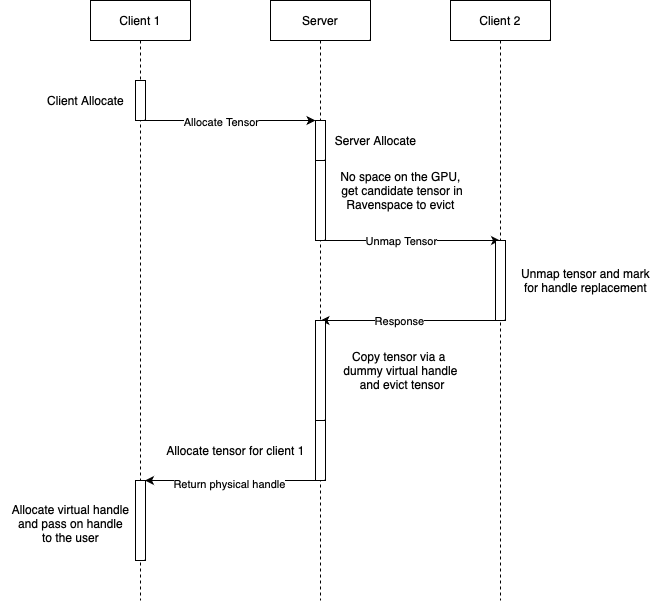
\includegraphics[height=8cm, width=8cm]{figures/Offloading.png}
	\caption{Sequence Diagram for Offloading}
\end{figure}
\FloatBarrier

Offloading is the process of moving tensors from the high memory tier to a lower memory tier, in this case from the GPU memory to RAM. When we have a situation where we do
not have any space for any new tensors requested by the client, we make space by offloading tensors from the
GPU memory to RAM. Our cache policy keeps track of the tensors and provides eviction candidates based on the policy (FIFO, LRU or Latency Aware). We then 
evict those tensors to allow the new tensor to allocate space in the GPU.

Post offloading when we need can get the tensor back when it is prefetched or via the GET call. In both the cases,
reallocation of the tensor happens and we get a new physical handle that the current virtual pointer does not point
to yet. Hence once we offload a tensor, we need to provide a callback to the client stating that the virtual pointer
for this tensor is now invalid and that we need to fetch the new tensor pointer again in order to give back to the user.

Hence, this way we are able to move tensors between the memory heirarchy and can them back up on demand.

\subsection{Prefetching}
\begin{figure}[!htbp]
	\centering
	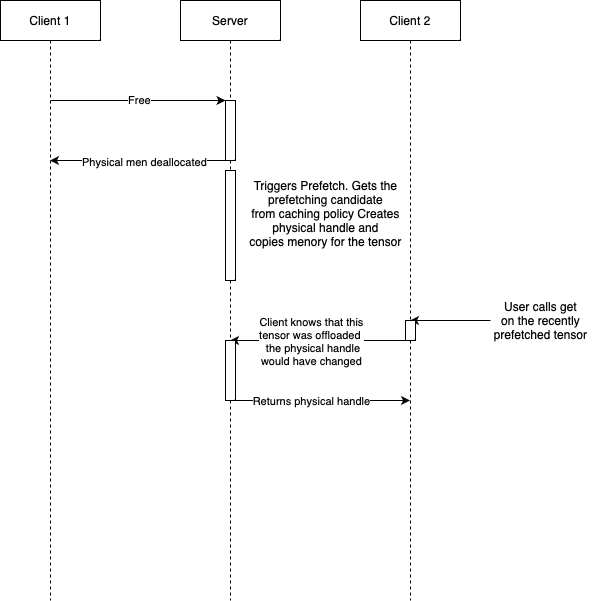
\includegraphics[height=8cm, width=8cm]{figures/Prefetch.png}
	\caption{Sequence Diagram for Prefetching}
\end{figure}
\FloatBarrier

Prefetching is the process in moving tensors back in to a higher memory tier from a lower memory tier, before they are needed. In our case it is moving tensors back into GPU memory from RAM.
This is done in alongside other computations in order to save time taken by the expensive IO call. When a tensor in the userspace is freed, it leaves us with space
that we can can use to store other tensors. Instead of allocating that tensor and copying data when the tensor is called we can do it beforehand based on a policy. Prefetching is also
crucial for our work since eager prefetching forms the basis of our goal of achieving high GPU memory utilization.

Whener a Free call is made on the on the server side, this includes all clients as well as all the other tensors we are intercepting, we run a defer a prefetch call. This calls the cache policy
which provides the prefetching candidates based on the policy and the size left. For latency aware caching for example, we always supply next access time for a tensor
in the PUT call itself. Hence we know when the tensor is going to be accessed next. Hence we can prefetch based on the next access time and prefetch the one with the earliest next access time.

When the client does a GET call on this tensor it the client knows to get the new handle fron the server since the older one was invalidated when the tensor was offloaded. But since we have already
added this tensor back to the GPU memory, we save on the expensive IO call and hence save time.


\section{Evaluation and Benchmarks}
After implementing memory harvesting on a single GPU, we wanted to see the overhead of various types caused in RavenStore.
We first compared the overhead of allocating and freeing tensors through RavenStore as compared with simple CUDAMalloc and CUDAFree
calls. Then we compared the overhead caused when assigning tensors to clients after creating them by creating virtual mapping through CUDA
Virtual Handles. Finally, we look into overhead caused when evicting tensors and offloading them to RAM, and then prefetching them from RAM.
We describe each of these evalutions in more detail in the following sections.

\subsection{Tensor Allocate/Free Overhead}

\subsection{Virtual Memory Overhead}
When creating CUDA Virtual Handle at client's end to manage tensors, virtual memory is created and mapping from
virtual address space to physical address space is done. We perform experiments to show that we get a virtual memory overhead
of 300 MBs for each client, and that memory overhead doesn't change as we increase the number of tensors, but it increases linearly
with the number of clients on the same GPU. The reason might be that underlying CUDA implementation creates page tables to map virtual address space
to physical address space, that page table might be occupying large amount of space in GPU.

\subsection{Eviction and Prefetching Overhead}
In section 5.1, we described the overhead of RavenStore when performing allocate and free API calls and compared that overhead with 
native CUDAMalloc and CUDAFree calls. In this section, we also describe the overhead we get when evicting tensors and prefetching them.
When evicting a tensor, two things happen: 1) Callback takes place to remove mapping on that tensor created by client, and 2) Server
offloads that tensor from GPU to RAM. Similarly, when prefetching tensor, Server has to create physical handle on the available space of
size required by tensor to be prefetched, and then tensor is moved back to GPU from RAM through CUDAMemcpy API.
To measure that, we create 2 processes. First process allocates the tensors of a specific size to fill the entire GPU memory. Once the entire GPU
memory space is filled, we launch second process which will also allocate tensors of same size. But since tensors of process 1 occupy space, they would
need to be evicted. This will cause overhead due to eviction. Furthermore, once we are done allocating all tensors of process 2, we will start freeing them.
Once we call free() for each tensor, tensors of first process which got evicted will now start coming back to GPU memory, i.e., prefetching for those
tensors will happen. This will help us measure overhead caused due to prefetching by comparing with time taken to simply free tensors without prefetching.
In the following subsections, we will describe the results of the above experiment.

\subsubsection{Eviction Overhead}
\subsubsection{Prefetching Overhead}

\section{Future Work}
Having implemented core components like eviction, enhancement of IPC, offloading tensors and prefetching, memory harvesting
on a single GPU is ready with few caveats as discussed later. We now plan
to extend to Multi-GPU setting with enhancements discussed in following subsection. 
Furthermore, with ravenstore APIs of get and put in place and heavy abstraction of what
happens inside ravenstore from client, there would be no changes needed from the client's end
in order to extend to multi-GPU design. In the following subsections we also discuss some pain points in the current implementation.

\subsection{Multi GPU Design}
We would extend to multi-GPU design with few more enhancements like enhancing 
eviction logic to also find the GPU to which the tensor can be offloaded instead
of simply offloading tensor to RAM, and in the scenario when no GPU is available
then we can simply offload to RAM. Furthermore, we would require additional data structures
to keep track of tensors stored across different GPUs so that we can fetch them to the GPU
where the client using those tensors is running. Once that is done, we won't require
any other changes to extend to multi-GPU design.

\subsection{PyTorch Binding}
Currently, clients explicitly need to make get() and put() calls to help RavenStore
manage tensors on their behalf. In order to train real world ML models written in PyTorch,
we would need to incorporate get/put calls during their training and inference. For that, we
plan to use torch.CUDAExtension. Implementation to extend PyTorch to work with RavenStore is complete,
however, we need to test our implementation and resolve any issues if needed.

\subsection{Current Limitations}
There are few limitations inherent in RavenStore due to limitations of CUDA APIs described as follows.
We plan to address these limitations, if possible, in future.
\subsubsection{Virtual Memory Overhead}
When creating CUDA Virtual Handles to manage CUDA tensors, additional space of approximately 300MBs is occupied 
for each client. We suspect that CUDA implementation creates page tables for each client to manage virtual memory.
So we will need to factor in that overhead caused when creating virtual memory.
\subsubsection{Latency in CUDAMemcpy}
During our experiments, after we evicted a particular tensor and called CUDAMemcpy to offload that tensor to RAM from GPU,
we couldn't immediately allocate new tensor of same size. We suspect that some time is needed for internal state of CUDA implementation
after we free the memory space in GPU. So after we imposed a time gap of 100 ms between eviction and allocation of new tensor, that error
went away.


\section{Conclusion}

Our focus on single-GPU memory harvesting serves as a foundational step, with extensions to multi-GPU scenarios. Through the demonstration of 
techniques such as eviction, prefetching of tensors, and the measurement of Ravenstore's overhead during model training, we provide practical insights into the viability and effectiveness of Memory Harvesting.

In summary, our Memory Harvesting technique represents a crucial advancement in addressing the challenges posed by limited GPU memory, offering a promising avenue 
for training large models despite stringent memory constraints. As deep learning continues to evolve, optimizing GPU memory utilization will play a pivotal role 
in unlocking the full potential of advanced models and pushing the boundaries of computational capabilities.

\section{Statement of Collaborator Contribution}
\subsection{Hersh Dhillon (AA, PJ)}
Conducted a literature review of existing work in the area of memory harvesting and caching and derived insights to set up the project.
Created a test bench for testing out physical and virtual memory mapping in CUDA.
Created the GET and PUT calls in both the client and the server side based on the inital code written by Anmol and created tests for it.
Worked on Pytorch Extension Bindings for the client side. This is still a work in progress since it still does not work as intended.
Created prefetching based on the older design (with client callbacks). The idea was to have all client data on the client and not let server make copies of data while taking out the tensors from RAM. However we decided to change our design to take care of MemCpy in the server side itself.
Removing data copying and callbacks from the client side for our design change. Changed the eviction mapping construct in the client to a ReplacedHandle construct to mark the tensors where the physical handle got changed due to offloading.

\subsection{Prakhar Jagwani (HD, AA)}
\subsection{Anmol Agarwal (PJ, HD)}
Anmol worked on the following things:
Help in fixing memory leak bug and raising PR with bug fix. Also resolved initial comments on the PR from Amey and Alan.
Helped in proposing initial FSM (Finite State Machine) describing states of tensors and transitions through client API calls
of allocate, get, put and free.
Implemented policies for caching and eviction such as FIFO, LRU, and Latency-Aware in C++ (ServerAllocator.cpp). 
Created dummy get/put API calls from Client side. The API calls were further enhanced by Hersh and Prakhar.
On suggestion of Alan and Amey, moved the implementation of eviction policies to Python through pybind11 (manager.py).
Modified CMAKE files to use pybind11 and further enhanced ServerAllocator.cpp code to make API calls in Python code.
Also implemented prefetching policies in Python by inconporating latency awareness using sortedcontainers library.
Helped in proposing new design to implement Prefetching mechanism and avoid callbacks to clients when doing prefetching.
Callbacks were earlier needed to map tensors from client's side and moving them back to GPU through virtual handle. But instead,
we decided to create virtual handle from Server to move tensors to GPU, hence avoiding callbacks.
Helped in integrating prefetching functionality inside ServerAllocator.cpp and resolve bugs related to prefetching mechanisms.
Collaborated with team members and helped in demo and project report (specifically in sections like Introduction, High Level Design,
Evaluation and Benchmarks, and Future Work).
Helped in designing experiment (more specifically experiment measuring Eviction and Prefetching Overhead).

\printbibliography

% \bibliographystyle{unsrtnat}
% \bibliography{references}  %%% Uncomment this line and comment out the ``thebibliography'' section below to use the external .bib file (using bibtex) .


%%% Uncomment this section and comment out the \bibliography{references} line above to use inline references.
% \begin{thebibliography}{1}

% 	\bibitem{kour2014real}
% 	George Kour and Raid Saabne.
% 	\newblock Real-time segmentation of on-line handwritten arabic script.
% 	\newblock In {\em Frontiers in Handwriting Recognition (ICFHR), 2014 14th
% 			International Conference on}, pages 417--422. IEEE, 2014.

% 	\bibitem{kour2014fast}
% 	George Kour and Raid Saabne.
% 	\newblock Fast classification of handwritten on-line arabic characters.
% 	\newblock In {\em Soft Computing and Pattern Recognition (SoCPaR), 2014 6th
% 			International Conference of}, pages 312--318. IEEE, 2014.

% 	\bibitem{keshet2016prediction}
% 	Keshet, Renato, Alina Maor, and George Kour.
% 	\newblock Prediction-Based, Prioritized Market-Share Insight Extraction.
% 	\newblock In {\em Advanced Data Mining and Applications (ADMA), 2016 12th International 
%                       Conference of}, pages 81--94,2016.

% \end{thebibliography}


\end{document}
